\chapter{Datos}
\label{chap:datos}

Este capítulo describe el conjunto de datos utilizado para entrenar el modelo, su selección y preparación, las variables construidas, la partición y los parámetros de entrenamiento, la adaptación de la telemetría del agente al esquema del conjunto de datos y el modelo de datos con el que el sistema persiste su estado.

\section{Conjunto de datos}
\label{sec:dataset}
El modelo se entrenó con CLUE-LDS (\emph{Cloud-based User Entity Behavior Analytics Log Data Set}) \parencite{Landauer2022, Landauer2022Dataset}. El conjunto contiene registros reales de actividad de los usuarios de una plataforma de almacenamiento y colaboración de archivos en la nube, seudonimizados mediante identificadores descriptivos. Abarca desde julio de 2017 hasta septiembre de 2022 y se distribuye bajo la licencia Creative Commons Atribución 4.0 (CC BY 4.0), que permite su uso con atribución a los autores.

Cada registro corresponde a un evento e incluye su tipo, la marca temporal, el identificador del usuario y su clase (nombre de usuario o dirección IP), parámetros específicos del tipo de evento y, cuando está disponible, la ubicación. El vocabulario comprende 44 tipos de evento propios de una plataforma de archivos compartidos, como accesos, creación y escritura de archivos, inicios de sesión y acceso a recursos compartidos públicamente.

El conjunto no incluye etiquetas que indiquen qué eventos corresponden a actividad maliciosa. Esta característica condiciona el entrenamiento, que es no supervisado, y la evaluación del modelo, que se presenta en la sección~\ref{sec:evaluacion-modelo}.

\section{Selección y preparación}
\label{sec:seleccion-datos}
El conjunto completo contiene 50\,522\,931 eventos y 920 usuarios identificados por nombre. Los usuarios se clasificaron según su volumen de actividad. No se descartaron eventos por su contenido: solo se clasificaron los usuarios. La tabla~\ref{tab:seleccion-datos} resume el resultado.

\begin{longtable}{>{\raggedright\arraybackslash}p{3.6cm}>{\raggedright\arraybackslash}p{4.4cm}>{\raggedright\arraybackslash}p{2.4cm}>{\raggedright\arraybackslash}p{2.0cm}}
	\caption{Clasificación de los usuarios del conjunto de datos}
	\label{tab:seleccion-datos}\\
	\hline
	\textbf{Categoría} & \textbf{Criterio} & \textbf{Eventos} & \textbf{Usuarios} \\
	\hline
	\endfirsthead
	\hline
	\textbf{Categoría} & \textbf{Criterio} & \textbf{Eventos} & \textbf{Usuarios} \\
	\hline
	\endhead
	Válidos & Entre 20 y 500\,000 eventos & 8\,494\,589 & 291 \\
	\hline
	Baja actividad & Menos de 20 eventos & 3\,000 & 617 \\
	\hline
	Cuentas de servicio & Más de 500\,000 eventos & 41\,879\,451 & 12 \\
	\hline
	Identificados por dirección IP & Usuario anónimo & 145\,891 & -- \\
	\hline
\end{longtable}

Las cuentas de servicio concentran el 83\,\% de los eventos y su comportamiento automatizado no representa la conducta de una persona, por lo que se excluyeron del entrenamiento. Los eventos identificados por dirección IP no pueden asociarse a un usuario y también se excluyeron. El mismo criterio se aplica en producción: estos casos quedan sin puntaje (RF-03).

\section{Variables y modelos}
\label{sec:variables-modelos}

Esta sección describe las variables que utiliza cada modelo, Isolation Forest y LSTM Autoencoder, y luego la partición de los datos y los parámetros de entrenamiento.

\subsection{Isolation Forest}
Isolation Forest evalúa cada día de actividad de cada usuario. Para cada par usuario-día, tomando el día calendario en UTC, se calculan ocho variables:
\begin{itemize}
	\item cantidad de eventos;
	\item cantidad de tipos de evento distintos;
	\item cantidad de países distintos;
	\item cantidad de eventos sobre archivos (acceso, creación y escritura);
	\item cantidad de eventos de autenticación;
	\item hora promedio de la actividad;
	\item proporción de eventos fuera de horario (antes de las 7 o después de las 20);
	\item entropía de la distribución de tipos de evento.
\end{itemize}

Se utilizaron los usuarios válidos y los de baja actividad: 908 usuarios y 61\,283 pares usuario-día. Las variables se estandarizaron antes del entrenamiento.

\subsection{LSTM Autoencoder}
El LSTM Autoencoder evalúa secuencias de 50 eventos consecutivos de cada usuario, sin solapamiento. Cada evento se representa con ocho variables: el tipo de evento codificado, la hora y el día de la semana en codificación cíclica (seno y coseno), el tiempo transcurrido desde el evento anterior del usuario, y dos indicadores de cambio, de país y de tipo de evento, respecto del evento previo. De los 291 usuarios válidos, 234 tienen al menos una secuencia completa, y se obtuvieron 169\,737 secuencias. Los 57 usuarios restantes tienen menos de 50 eventos.

\subsection{Partición y parámetros}
La tabla~\ref{tab:entrenamiento} resume la partición de los datos y los parámetros de cada modelo.

\begin{longtable}{>{\raggedright\arraybackslash}p{3.0cm}>{\raggedright\arraybackslash}p{5.5cm}>{\raggedright\arraybackslash}p{5.6cm}}
	\caption{Partición de los datos y parámetros de entrenamiento}
	\label{tab:entrenamiento}\\
	\hline
	\textbf{Aspecto} & \textbf{Isolation Forest} & \textbf{LSTM Autoencoder} \\
	\hline
	\endfirsthead
	\hline
	\textbf{Aspecto} & \textbf{Isolation Forest} & \textbf{LSTM Autoencoder} \\
	\hline
	\endhead
	Unidad de análisis & Usuario-día & Secuencia de 50 eventos \\
	\hline
	Partición & Temporal: entrenamiento hasta el 2 de agosto de 2021 (cuantil 0,8 de las fechas), prueba posterior & Por usuario, con semilla fija: 70\,\% entrenamiento, 15\,\% validación y 15\,\% prueba \\
	\hline
	Tamaño & 49\,048 usuario-días de entrenamiento y 12\,235 de prueba & 163, 35 y 36 usuarios; 111\,742, 20\,741 y 37\,254 secuencias \\
	\hline
	Parámetros & 200 árboles, contaminación de 0,02 & Codificador LSTM(64) y LSTM(32), decodificador simétrico, \emph{embedding} de dimensión 8; 67\,375 parámetros \\
	\hline
	Entrenamiento & -- & Error cuadrático medio, optimizador Adam, lotes de 128, detención temprana en la época 22 (pérdida de validación 0,0805) \\
	\hline
	Criterio de anomalía & Puntaje de aislamiento según la contaminación & Error de reconstrucción mayor al percentil 95 del entrenamiento (0,1368) \\
	\hline
\end{longtable}

El puntaje híbrido combina ambos modelos con un peso de 0,5 cada uno y aplica un decaimiento temporal con una vida media de 3 días. Los umbrales por defecto de los niveles son 40, 70 y 90. Los dos modelos se particionaron con criterios distintos: la partición temporal evalúa la capacidad de Isolation Forest de generalizar hacia el futuro, mientras que la partición por usuario evalúa la del LSTM sobre usuarios no vistos. Como consecuencia, solo 15 usuarios están en el conjunto de prueba de ambos modelos, lo que limita la evaluación conjunta (sección~\ref{sec:evaluacion-modelo}).

\section{Adaptación de la telemetría del agente}
\label{sec:mapeo-agente}
El agente observa un \emph{endpoint} Windows, mientras que el modelo se entrenó con eventos de una plataforma de archivos en la nube. Para que el modelo pueda evaluar la telemetría del agente sin reentrenarse, cada señal del sistema operativo se traduce a un tipo de evento del vocabulario de CLUE-LDS. La tabla~\ref{tab:mapeo-agente} presenta esa correspondencia y su efecto sobre las variables de Isolation Forest.

\begin{longtable}{>{\raggedright\arraybackslash}p{3.6cm}>{\raggedright\arraybackslash}p{3.8cm}>{\raggedright\arraybackslash}p{6.7cm}}
	\caption{Correspondencia entre las señales del agente y los tipos de evento del conjunto de datos}
	\label{tab:mapeo-agente}\\
	\hline
	\textbf{Señal del sistema operativo} & \textbf{Tipo de evento} & \textbf{Aporte a las variables de Isolation Forest} \\
	\hline
	\endfirsthead
	\hline
	\textbf{Señal del sistema operativo} & \textbf{Tipo de evento} & \textbf{Aporte a las variables de Isolation Forest} \\
	\hline
	\endhead
	Archivo creado & \texttt{file\_\allowbreak{}created} & Todas, incluida la cantidad de eventos sobre archivos \\
	\hline
	Archivo modificado & \texttt{file\_\allowbreak{}written} & Todas, incluida la cantidad de eventos sobre archivos \\
	\hline
	Archivo renombrado & \texttt{file\_\allowbreak{}renamed} & Variables generales; no suma a los eventos sobre archivos \\
	\hline
	Archivo borrado & \texttt{file\_\allowbreak{}deleted} & Variables generales; no suma a los eventos sobre archivos \\
	\hline
	Proceso o aplicación iniciado & \texttt{app\_\allowbreak{}enabled} & Variables generales; no suma a ningún conteo específico \\
	\hline
	Proceso o aplicación finalizado & \texttt{app\_\allowbreak{}disabled} & Variables generales; no suma a ningún conteo específico \\
	\hline
	Conexión de red saliente & \texttt{public\_\allowbreak{}share\_\allowbreak{}accessed} & Variables generales; no suma a ningún conteo específico \\
	\hline
	Inicio del agente & \texttt{login\_\allowbreak{}successful} & Todas, incluida la cantidad de eventos de autenticación \\
	\hline
	Detención del agente & \texttt{logout\_\allowbreak{}occured} & Variables generales \\
	\hline
\end{longtable}

En esta tabla, las variables generales son la cantidad de eventos, la variedad de tipos, la hora promedio, la proporción fuera de horario y la entropía. El LSTM utiliza para todos los eventos el tipo codificado, la información temporal y los indicadores de cambio.

Esta correspondencia es una decisión de diseño que permite reutilizar un modelo entrenado con datos reales en lugar de uno entrenado con datos sintéticos, y tiene limitaciones que se declaran explícitamente:
\begin{itemize}
	\item Ninguno de los tipos utilizados describe de forma nativa un proceso o una conexión de red. Los eventos de aplicación de CLUE-LDS se refieren a aplicaciones de la propia plataforma, y el acceso a un recurso compartido públicamente es una aproximación semántica para una conexión saliente.
	\item El modelo evalúa el tipo de evento y su distribución temporal, no el nombre del proceso, el archivo o el destino de la conexión. Por eso, no reconoce por sí mismo un proceso inusual ni un destino de red sospechoso: detecta cambios en el volumen, la variedad y el horario de la actividad.
	\item El 99,946\,\% de los eventos utilizados tiene el país registrado como desconocido, por lo que la variable de cambio de país casi no varía en el entrenamiento.
	\item El indicador de dirección local que envía el agente describe la red del equipo y no la de la conexión. El modelo no lo utiliza.
\end{itemize}

La forma de eliminar esta transferencia de dominio es reentrenar el modelo con telemetría propia de \emph{endpoints}, recolectada por el agente durante un período de operación real. El mecanismo de reentrenamiento periódico ya incorpora los eventos crudos recibidos como insumo.

\section{Modelo de datos}
\label{sec:modelo-datos}
El sistema persiste su información en dos almacenes con funciones distintas. Redis guarda el estado operativo que se lee y actualiza en cada evento, y PostgreSQL guarda el historial y los registros que deben conservarse.

\subsection{Modelo relacional}
La base de datos relacional tiene siete tablas, presentadas en la tabla~\ref{tab:tablas-postgres}. Las figuras~\ref{fig:er-scoring} y~\ref{fig:er-config} muestran su estructura.

\begin{longtable}{>{\raggedright\arraybackslash}p{4.6cm}>{\raggedright\arraybackslash}p{9.5cm}}
	\caption{Tablas del modelo relacional}
	\label{tab:tablas-postgres}\\
	\hline
	\textbf{Tabla} & \textbf{Contenido} \\
	\hline
	\endfirsthead
	\hline
	\textbf{Tabla} & \textbf{Contenido} \\
	\hline
	\endhead
	\texttt{historial\_\allowbreak{}scores} & Una fila por usuario y día cerrado: puntaje, nivel, cobertura, acción sugerida, explicación y motivo. \\
	\hline
	\texttt{eventos\_\allowbreak{}crudos} & Cada evento recibido, sin puntaje, con su \emph{hash} y el \emph{hash} del evento anterior del mismo usuario. \\
	\hline
	\texttt{drift\_\allowbreak{}alerts} & Corrimientos significativos de la línea base personal, con el modelo afectado y las variables involucradas. \\
	\hline
	\texttt{historial\_\allowbreak{}politicas} & Auditoría de cambios de configuración, con los valores anteriores y nuevos y el actor. \\
	\hline
	\texttt{historial\_\allowbreak{}reentrenamientos} & Registro de cada reentrenamiento: fecha, cantidad de eventos, variación de las métricas y actor. \\
	\hline
	\texttt{metricas\_\allowbreak{}modelo} & Métrica de cada modelo entrenado y cuál es el vigente. \\
	\hline
	\texttt{historial\_\allowbreak{}agent\_\allowbreak{}keys} & Altas y revocaciones de las claves de los agentes. \\
	\hline
\end{longtable}

\begin{figure}[ht]
	\centering
	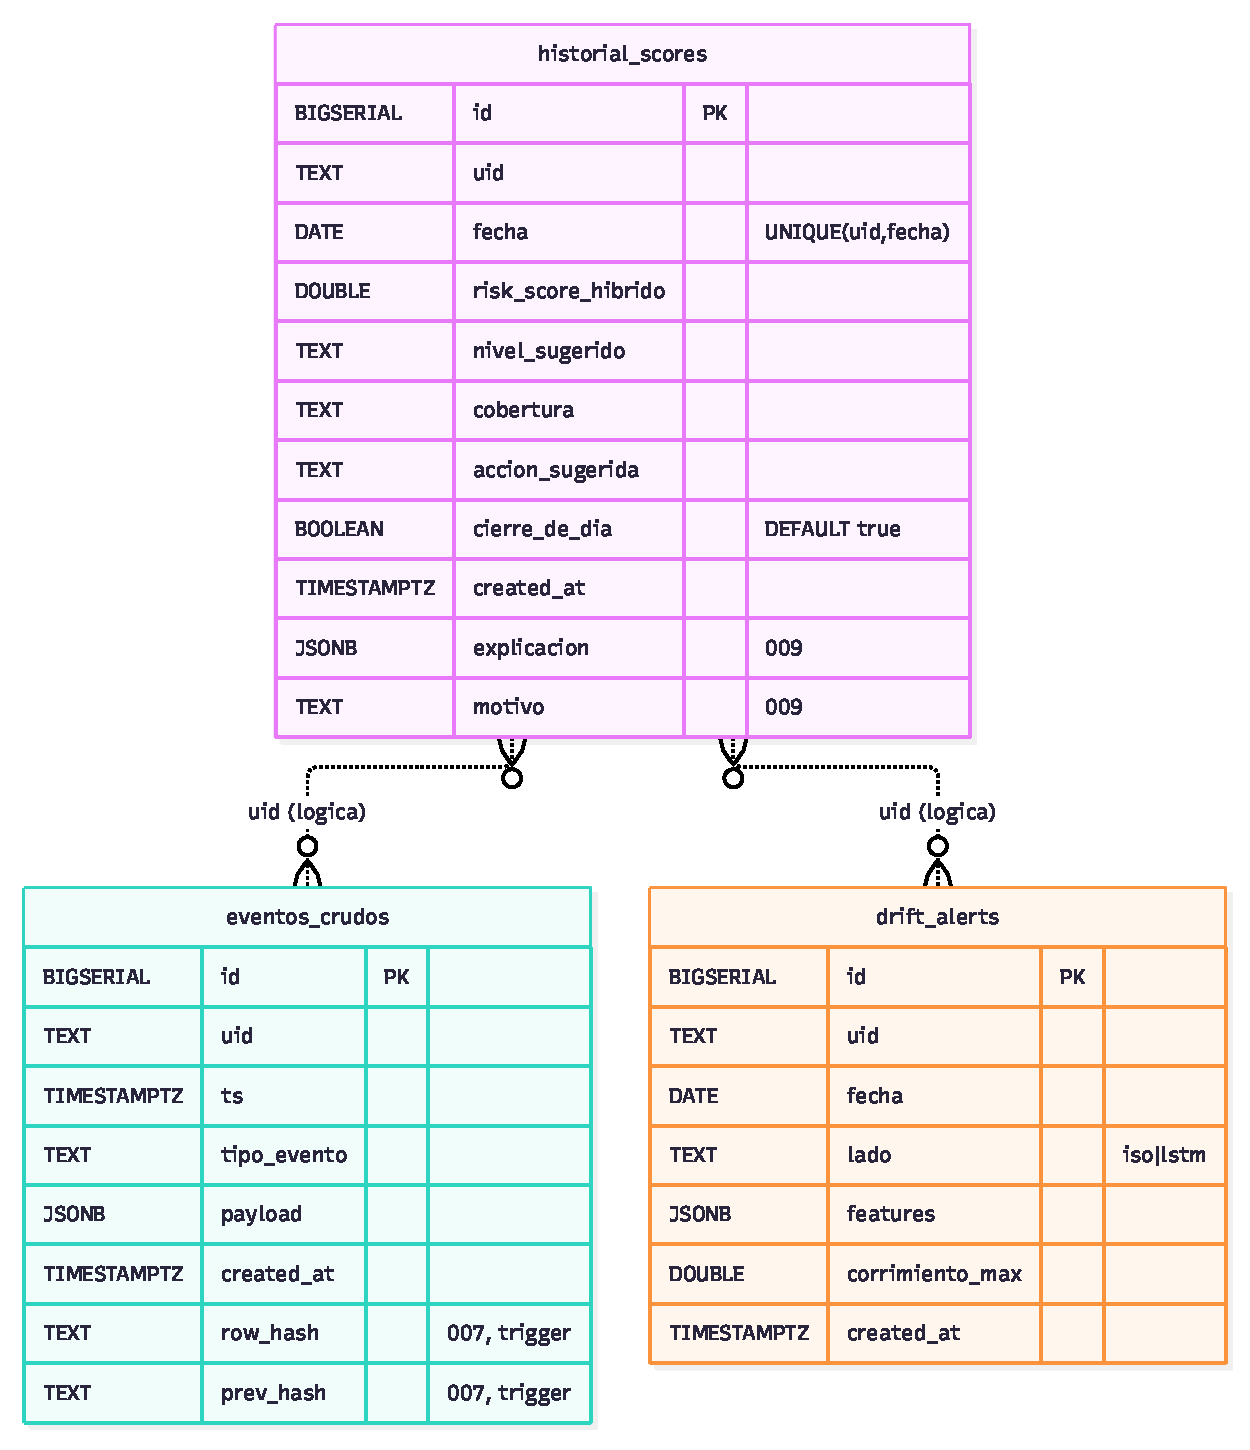
\includegraphics[width=13.5cm]{images/diagramas/v75/er_postgres_scoring_eventos.pdf}
	\caption{Modelo relacional: puntajes, eventos crudos y alertas de corrimiento}
	\label{fig:er-scoring}
\end{figure}

\begin{figure}[ht]
	\centering
	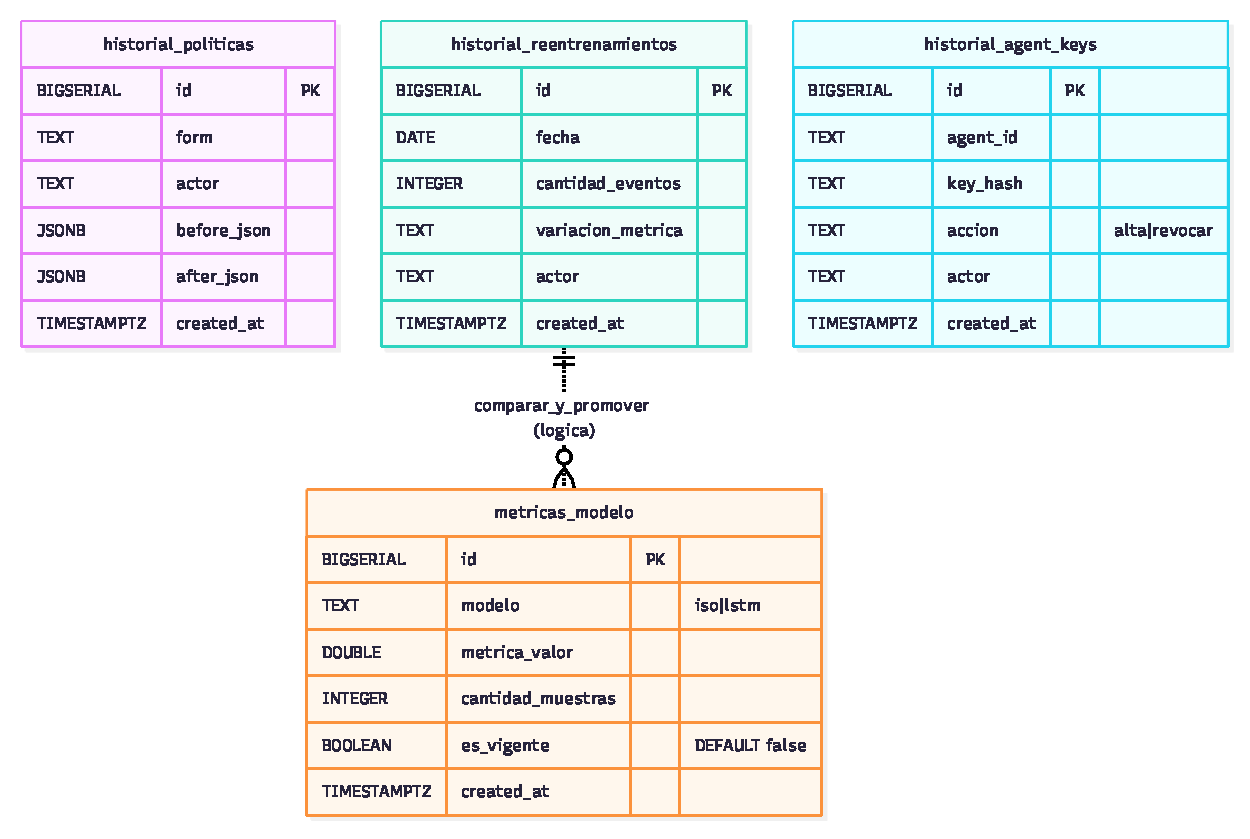
\includegraphics[width=13.5cm]{images/diagramas/v75/er_postgres_config_modelos.pdf}
	\caption{Modelo relacional: auditoría, reentrenamientos, métricas y claves de agentes}
	\label{fig:er-config}
\end{figure}

Las tablas no tienen claves foráneas: se relacionan lógicamente a través del identificador de usuario. Esta decisión simplifica la persistencia, que es tolerante a fallas: si la base de datos no está disponible, la evaluación de eventos continúa. Como contrapartida, la integridad referencial queda a cargo de la aplicación, por ejemplo la regla de un único modelo vigente por tipo. Seis de las siete tablas tienen activada la seguridad a nivel de fila, de modo que no pueden leerse desde la API pública de la plataforma de base de datos, y solo la API del sistema accede con sus credenciales. La tabla \texttt{historial\_\allowbreak{}scores} no tiene esta protección activada; su incorporación queda registrada como mejora pendiente.

La integridad de los eventos crudos se garantiza con una cadena de \emph{hashes} por usuario. Un disparador de la base de datos calcula, antes de cada inserción, el \emph{hash} SHA-256 de la fila a partir de sus campos y del \emph{hash} de la fila anterior del mismo usuario. Si se modifica o elimina una fila, la cadena deja de verificarse a partir de ese punto.

\subsection{Modelo no relacional}
Redis almacena catorce tipos de clave, agrupados en la tabla~\ref{tab:claves-redis}. Ninguna utiliza la expiración nativa de Redis: cuando una clave debe vencer, la fecha de vencimiento se guarda dentro del valor y se verifica al leerla. Esta decisión permite ejecutar las pruebas con un Redis simulado en memoria con el mismo comportamiento. El estado de cada usuario se actualiza con transacciones optimistas, con reintentos ante escrituras concurrentes, lo que sostiene el requerimiento RNF-14.

\begin{longtable}{>{\raggedright\arraybackslash}p{3.4cm}>{\raggedright\arraybackslash}p{7.2cm}>{\raggedright\arraybackslash}p{3.5cm}}
	\caption{Claves de Redis agrupadas por función}
	\label{tab:claves-redis}\\
	\hline
	\textbf{Grupo} & \textbf{Contenido} & \textbf{Vigencia} \\
	\hline
	\endfirsthead
	\hline
	\textbf{Grupo} & \textbf{Contenido} & \textbf{Vigencia} \\
	\hline
	\endhead
	Estado del usuario & Estado de \emph{scoring} completo: continuidad, acumulados de cada modelo, línea base personal, último puntaje, nivel, acción, explicación, contexto IAM y última confirmación del agente & Permanente \\
	\hline
	Eventos recientes & Lista acotada de los últimos eventos evaluados de cada usuario & Permanente, con tope configurable \\
	\hline
	Intervalo de notificación & Momento hasta el cual no se reenvía un correo para el usuario & 10 minutos \\
	\hline
	Deduplicación & Respuesta ya calculada para un evento reenviado & 6 horas \\
	\hline
	Claves de agentes & \emph{Hash} de cada clave con el identificador del agente y su estado & Hasta su revocación \\
	\hline
	Caché IAM & Rol y departamento del usuario, y \emph{token} de acceso al proveedor & 30 minutos para el rol (1 minuto ante fallas); el \emph{token}, según su vencimiento \\
	\hline
	Configuración & Umbrales, acciones por nivel, niveles que notifican, destinatarios, reentrenamiento, límite de eventos recientes y umbral de aprendizaje & Permanente \\
	\hline
\end{longtable}

\section{Síntesis}
\label{sec:sintesis-datos}
El modelo se entrenó con 8,5 millones de eventos reales de 291 usuarios, sin etiquetas. Isolation Forest trabaja sobre variables diarias y el LSTM sobre secuencias de 50 eventos. La telemetría del agente se traduce al vocabulario del conjunto de datos, lo que permite usar un modelo entrenado con datos reales, a costa de una transferencia de dominio que limita qué patrones puede reconocer. El sistema separa el estado operativo, en Redis, del historial auditable, en PostgreSQL, y protege la integridad de los eventos crudos con una cadena de \emph{hashes}.
